\documentclass[prb,preprint]{revtex4-1} 
% The line above defines the type of LaTeX document.
% Note that AJP uses the same style as Phys. Rev. B (prb).

\usepackage{amsmath}  % needed for \tfrac, \bmatrix, etc.
\usepackage{amsfonts} % needed for bold Greek, Fraktur, and blackboard bold
\usepackage{graphicx} % needed for figures
\usepackage{tabularx}

\begin{document}

\title{Optical Pumping of Rubidium OP1-A}
% In a long title you can use \\ to force a line break at a certain location.

\author{Yumeng Melody Cao}
\email{mcao@smith.edu} 
\affiliation{Department of Physics, Smith College, Northampton, MA 01063}
\author{He Claudia Yun}
\email{hyun@smith.edu}
\affiliation{Department of Physics, Smith College, Northampton, MA 01063}

% See the REVTeX documentation for more examples of author and affiliation lists.

\date{\today}

%____________abstract____________________________________________

\begin{abstract}

\end{abstract}

\maketitle 

%____________Introduction____________________________________________
\section{Introduction}

In our experiment, optical pumping is conducted where light is used to "pump" electrons from a lower energy level in Rubidium atoms to higher energy levels achieving population inversion. This process of optical 

%____________Experiment____________________________________________
\section{Experiment}

To implement the optical pumping process, we used the apparatus shown in Fig. 
\ref{exp}, manufactured by TeachSpin Inc. \\

\begin{figure}[h]
\centering
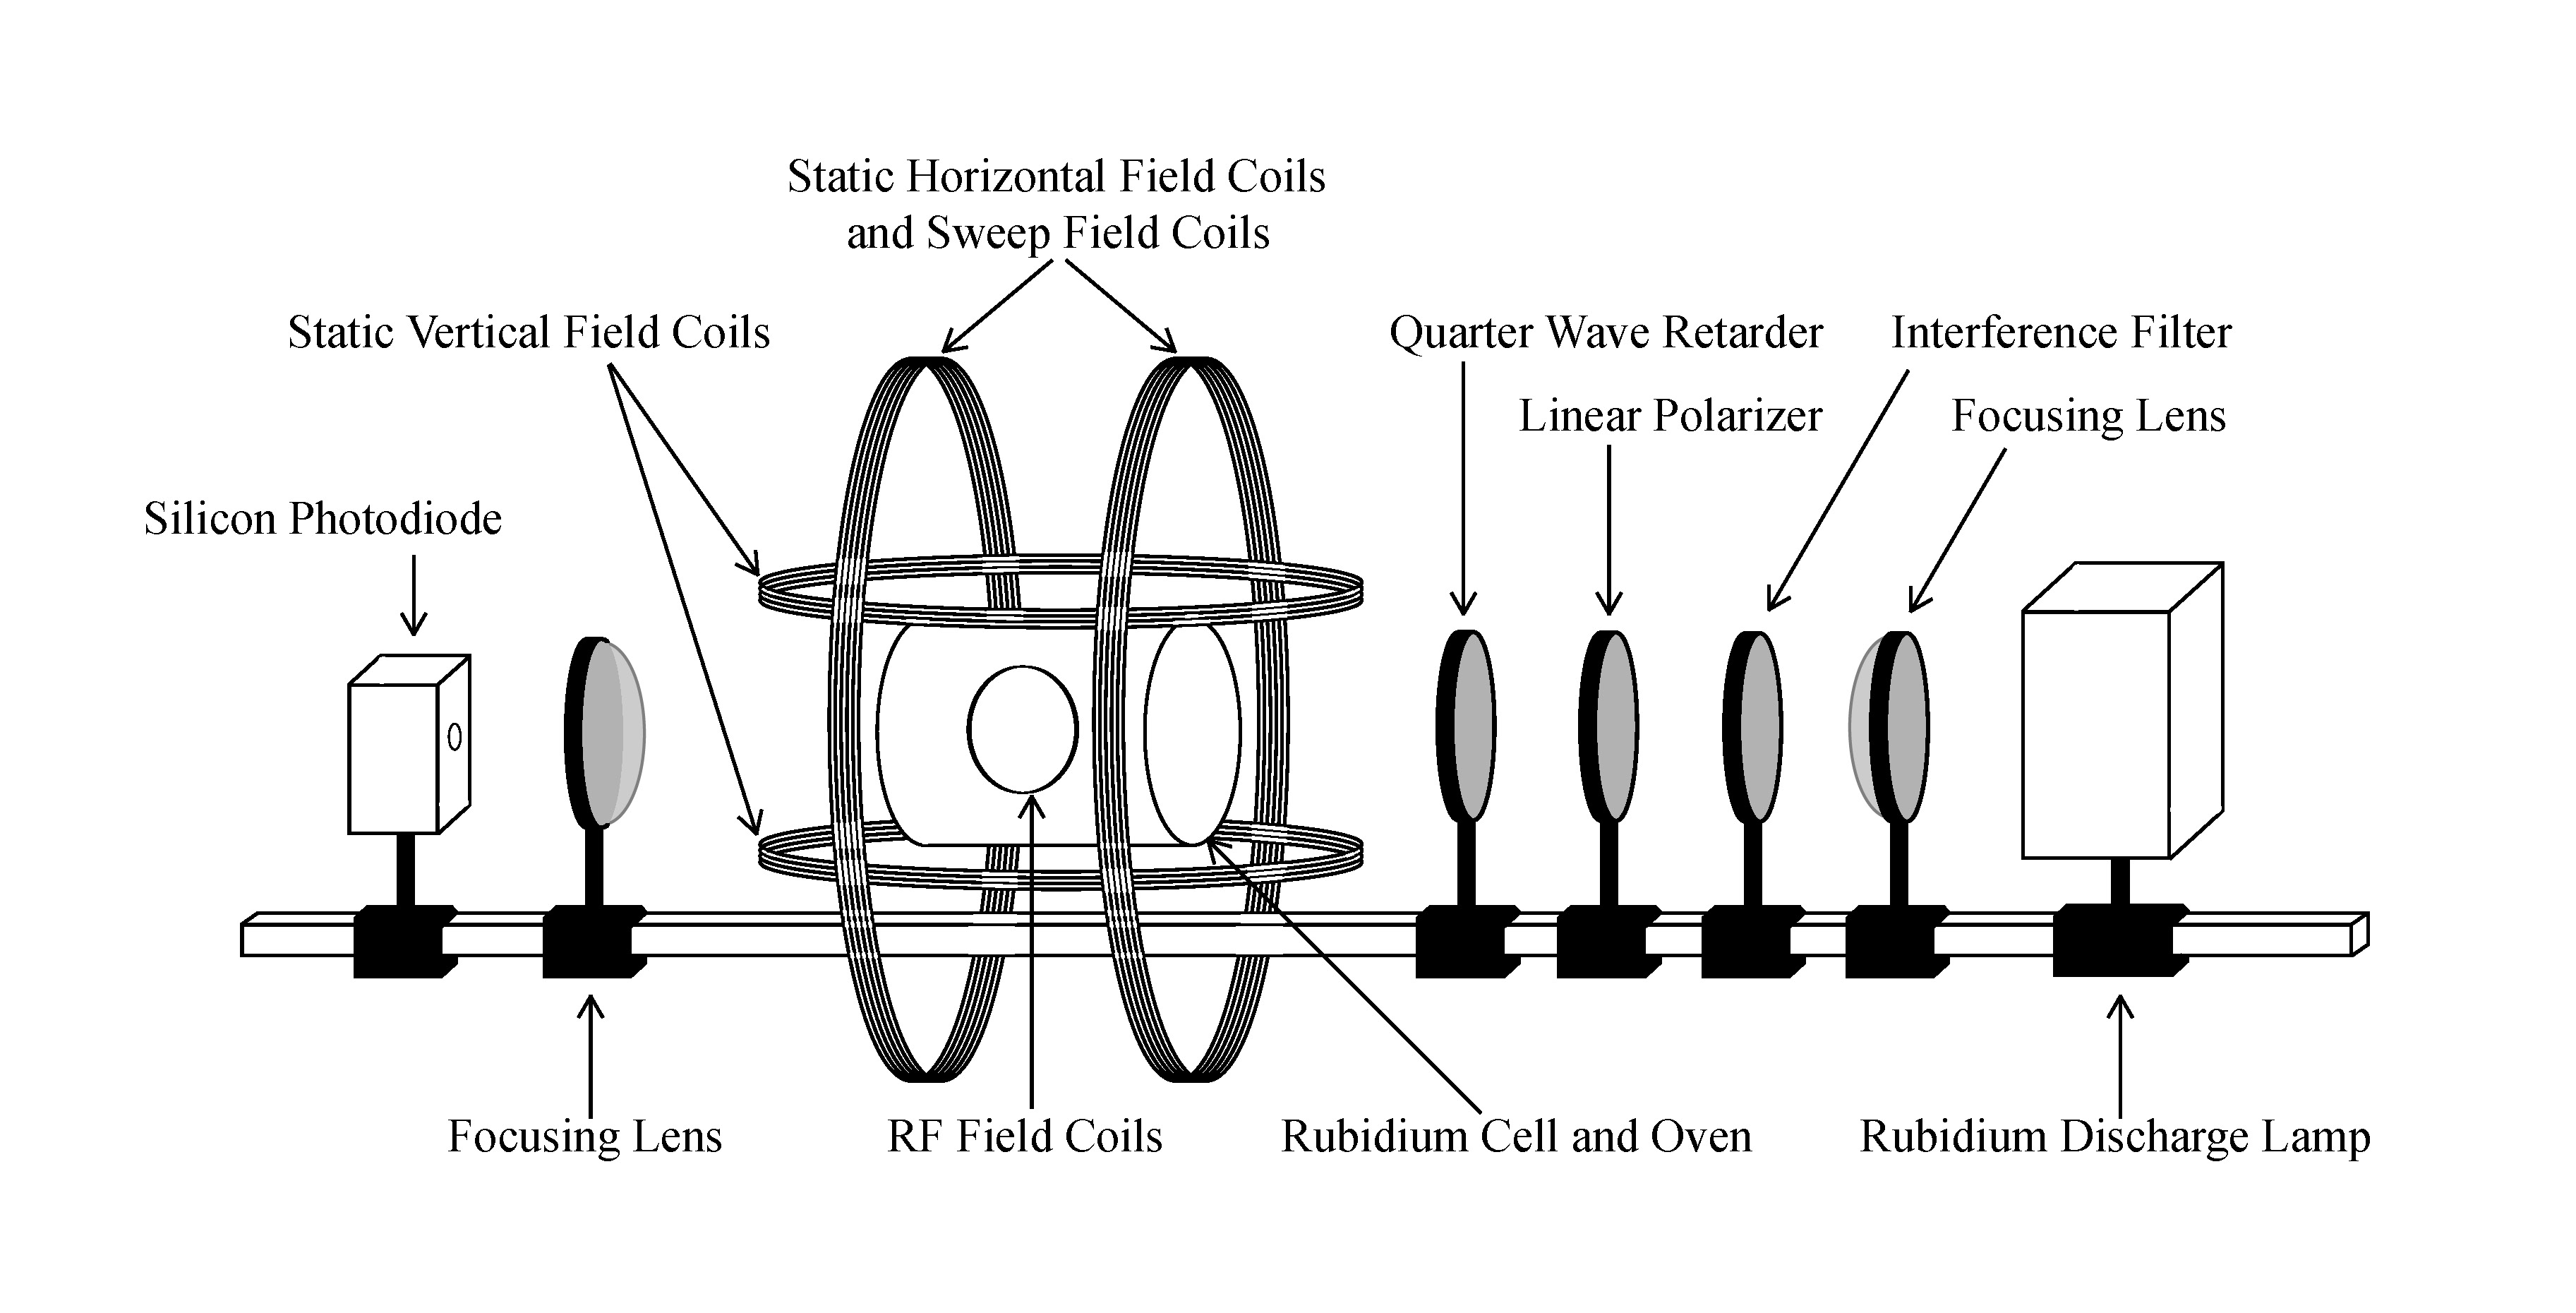
\includegraphics[width=18cm]{exp.jpg}
\caption{Optical pumping of Rubidium apparatus}
\label{exp}
\end{figure}

On the right side of the optical rail, the interference filter limits the bandwidth of light with a pass band of 790 nm to 830 nm, and the linear polarizer and quarter wave retarder convert the light from random polarization to circular polarization. The circular polarized light mandates only $\delta M=+1$ electric dipole transitions in the atom.The Helmholtz coils provide the magnetic fields, are driven by dial controlled variable voltage dividers, and are monitored by two Agilent 34410 digital multimeters and a Tektronix 2024B oscilloscope. The left side of the optical rail measures the intensity of light passing through the sample which in effect allows us to see when the sample is driven out of the optically pumped state. This signal is also monitored by the oscilloscope. The RF field coils are driven by an HP33120A function generator and drive the sample out of the optically pumped state when the sweep field is at resonance.


%____________Results____________________________________________
\section{Results}

\begin{figure}[h]
\centering
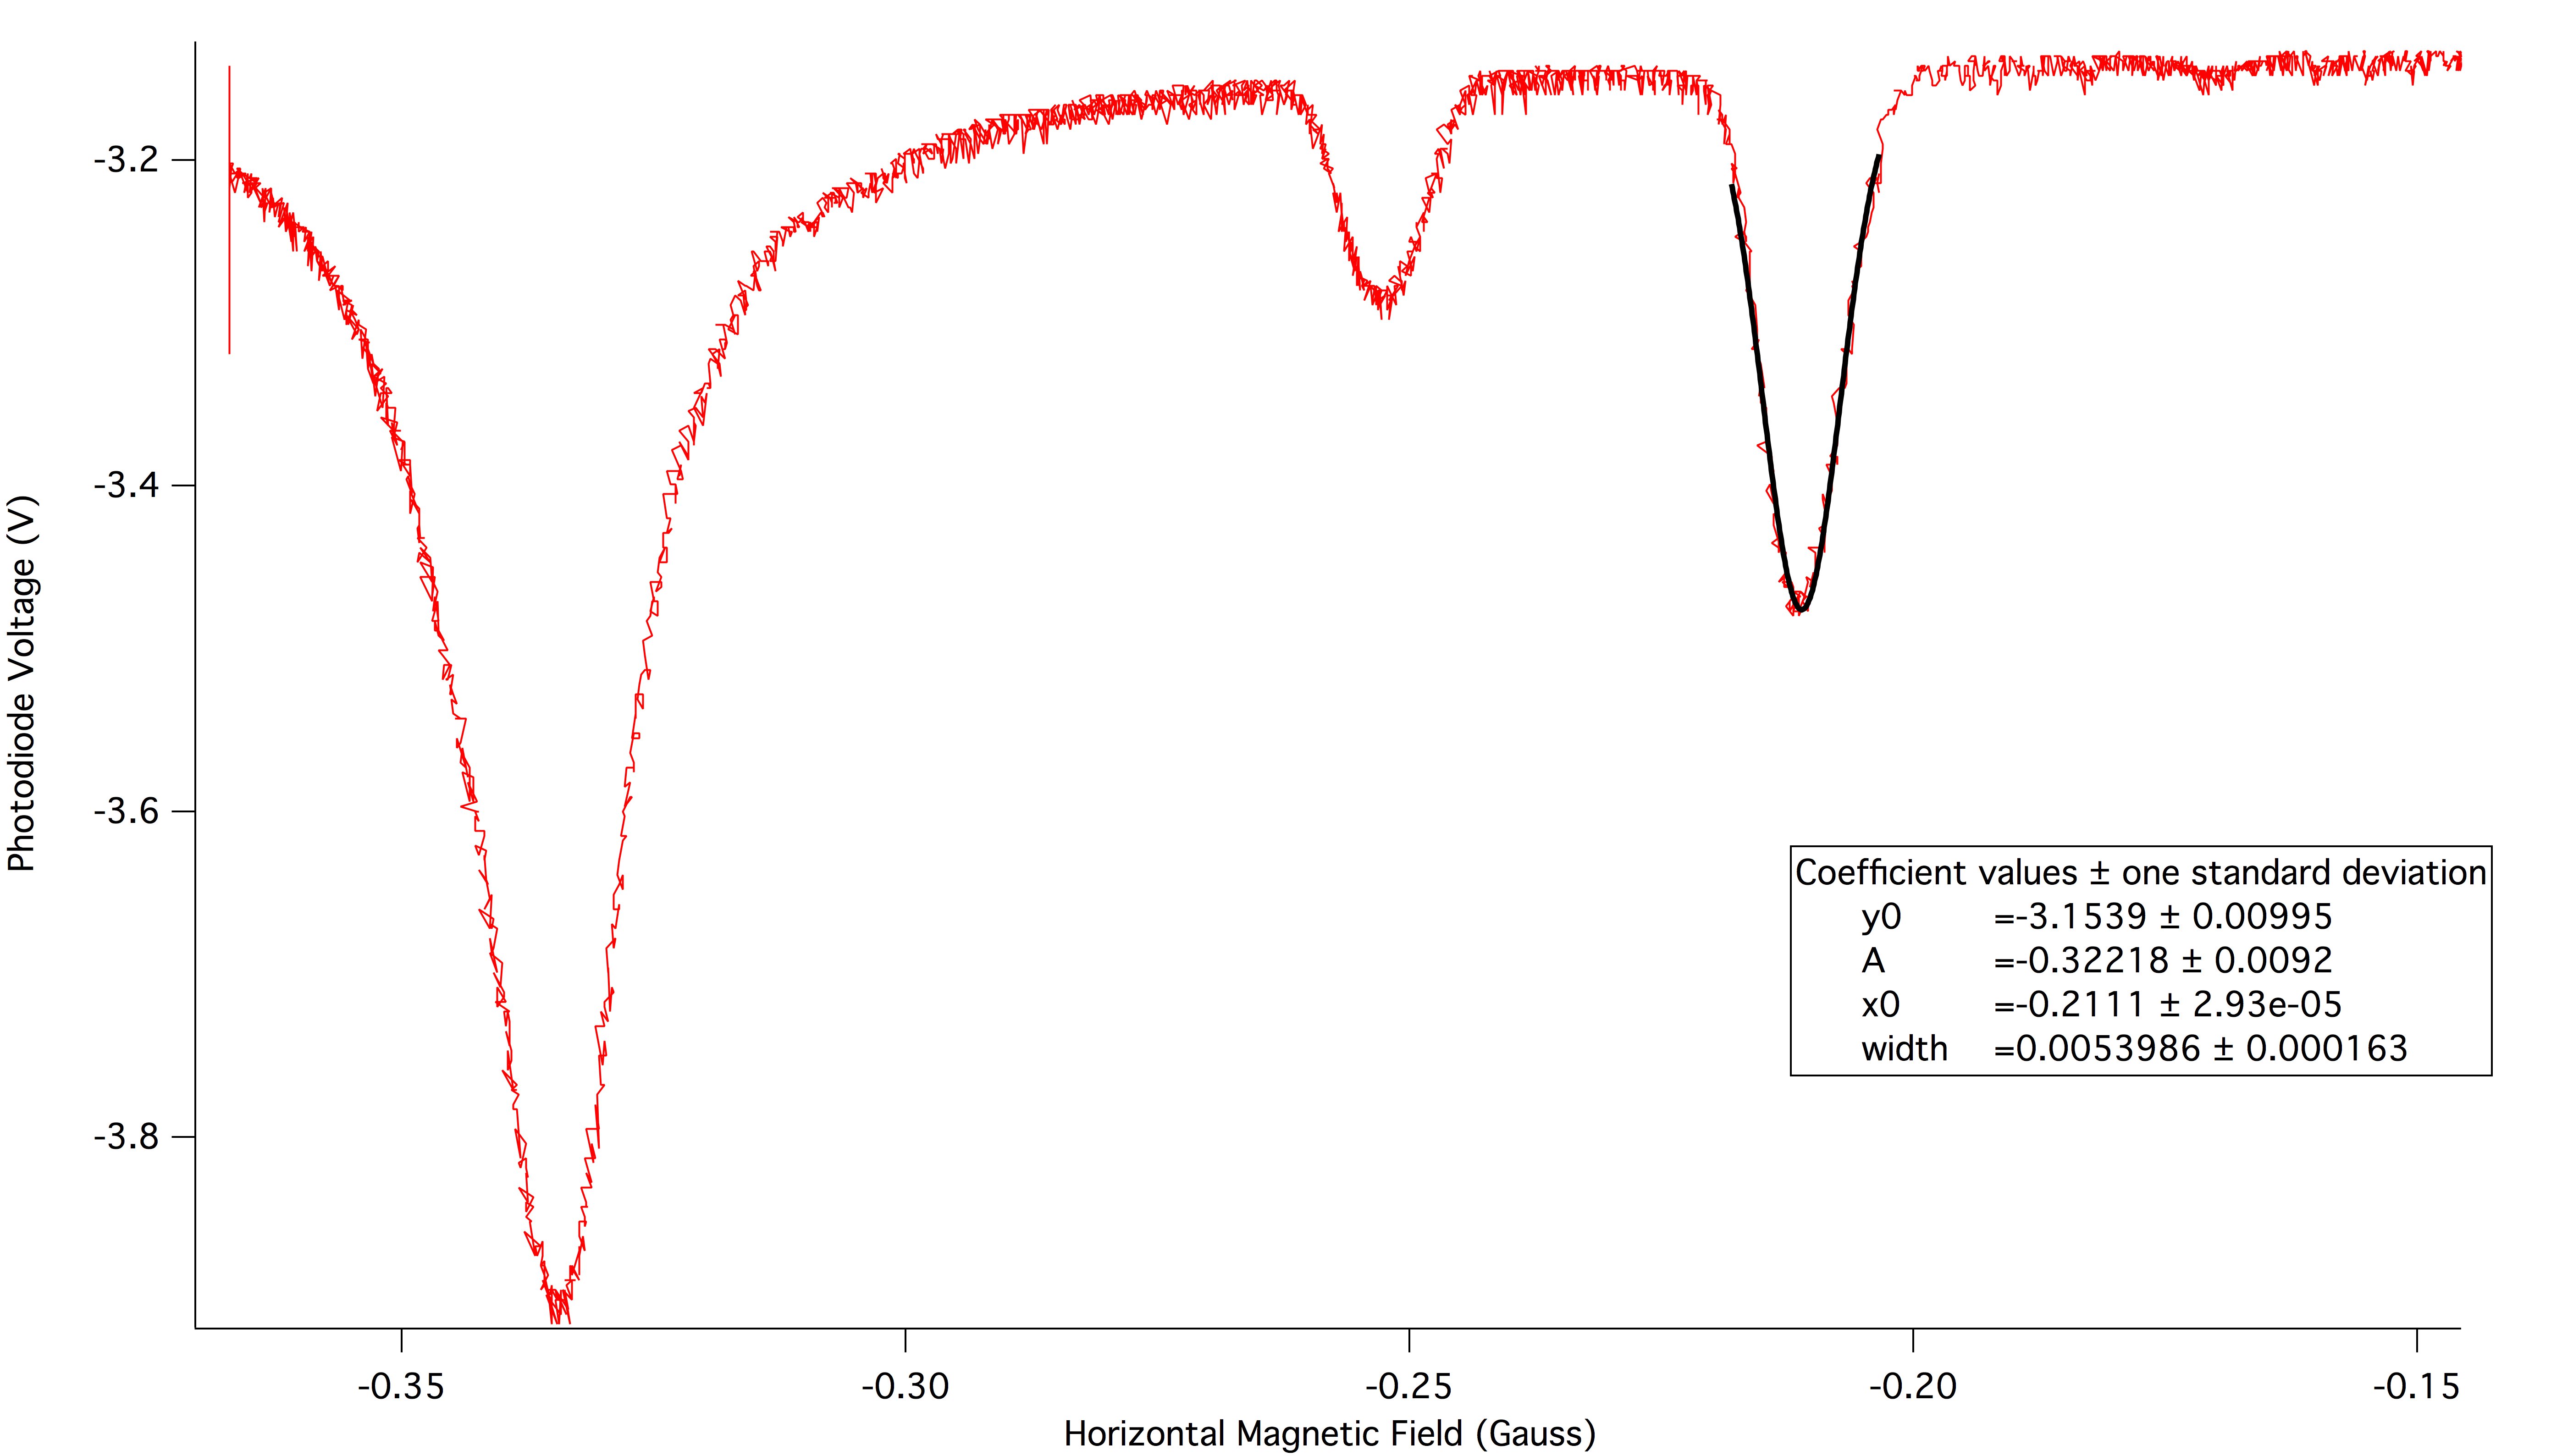
\includegraphics[width=18cm]{graph0}
\caption{Photo-voltage versus magnetic field strength at 100 kHz. The left trough is the zero field resonance, the middle trough is RF absorption for $^87$Rb and the right trough is for Rb.}
\label{exp}
\end{figure}


\begin{figure}[h]
\centering
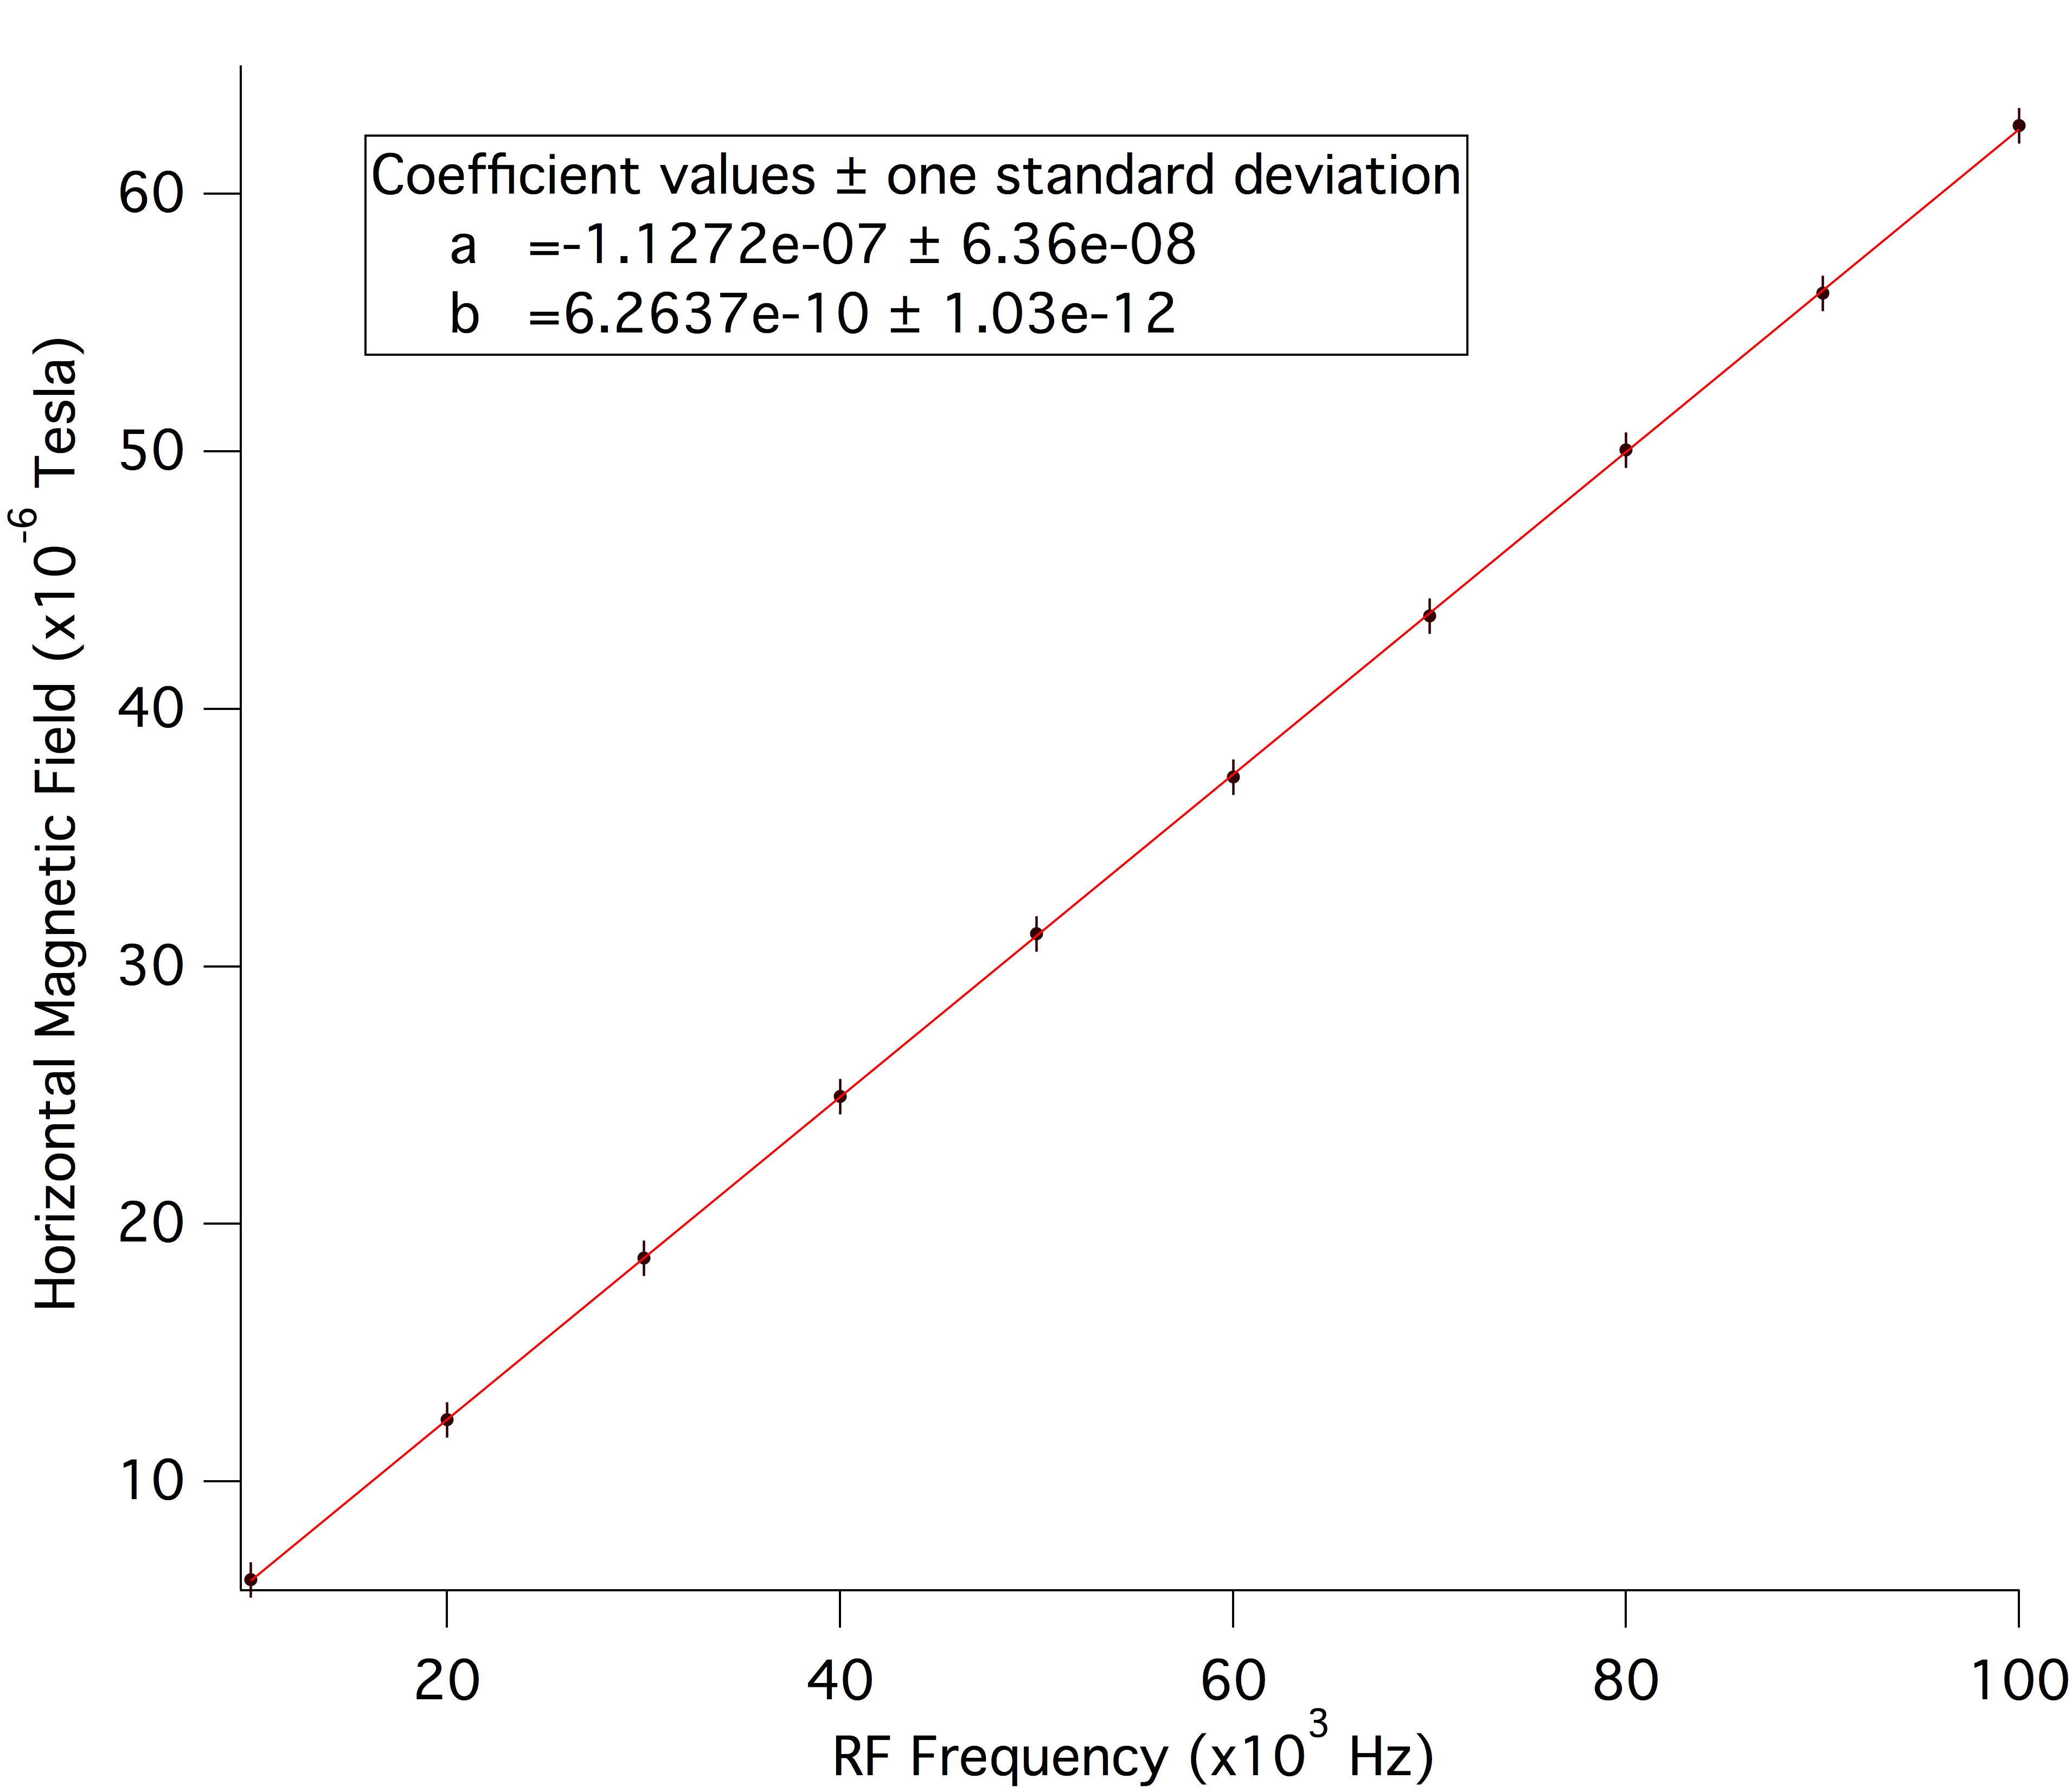
\includegraphics[width=8cm]{85vsFreq.png}
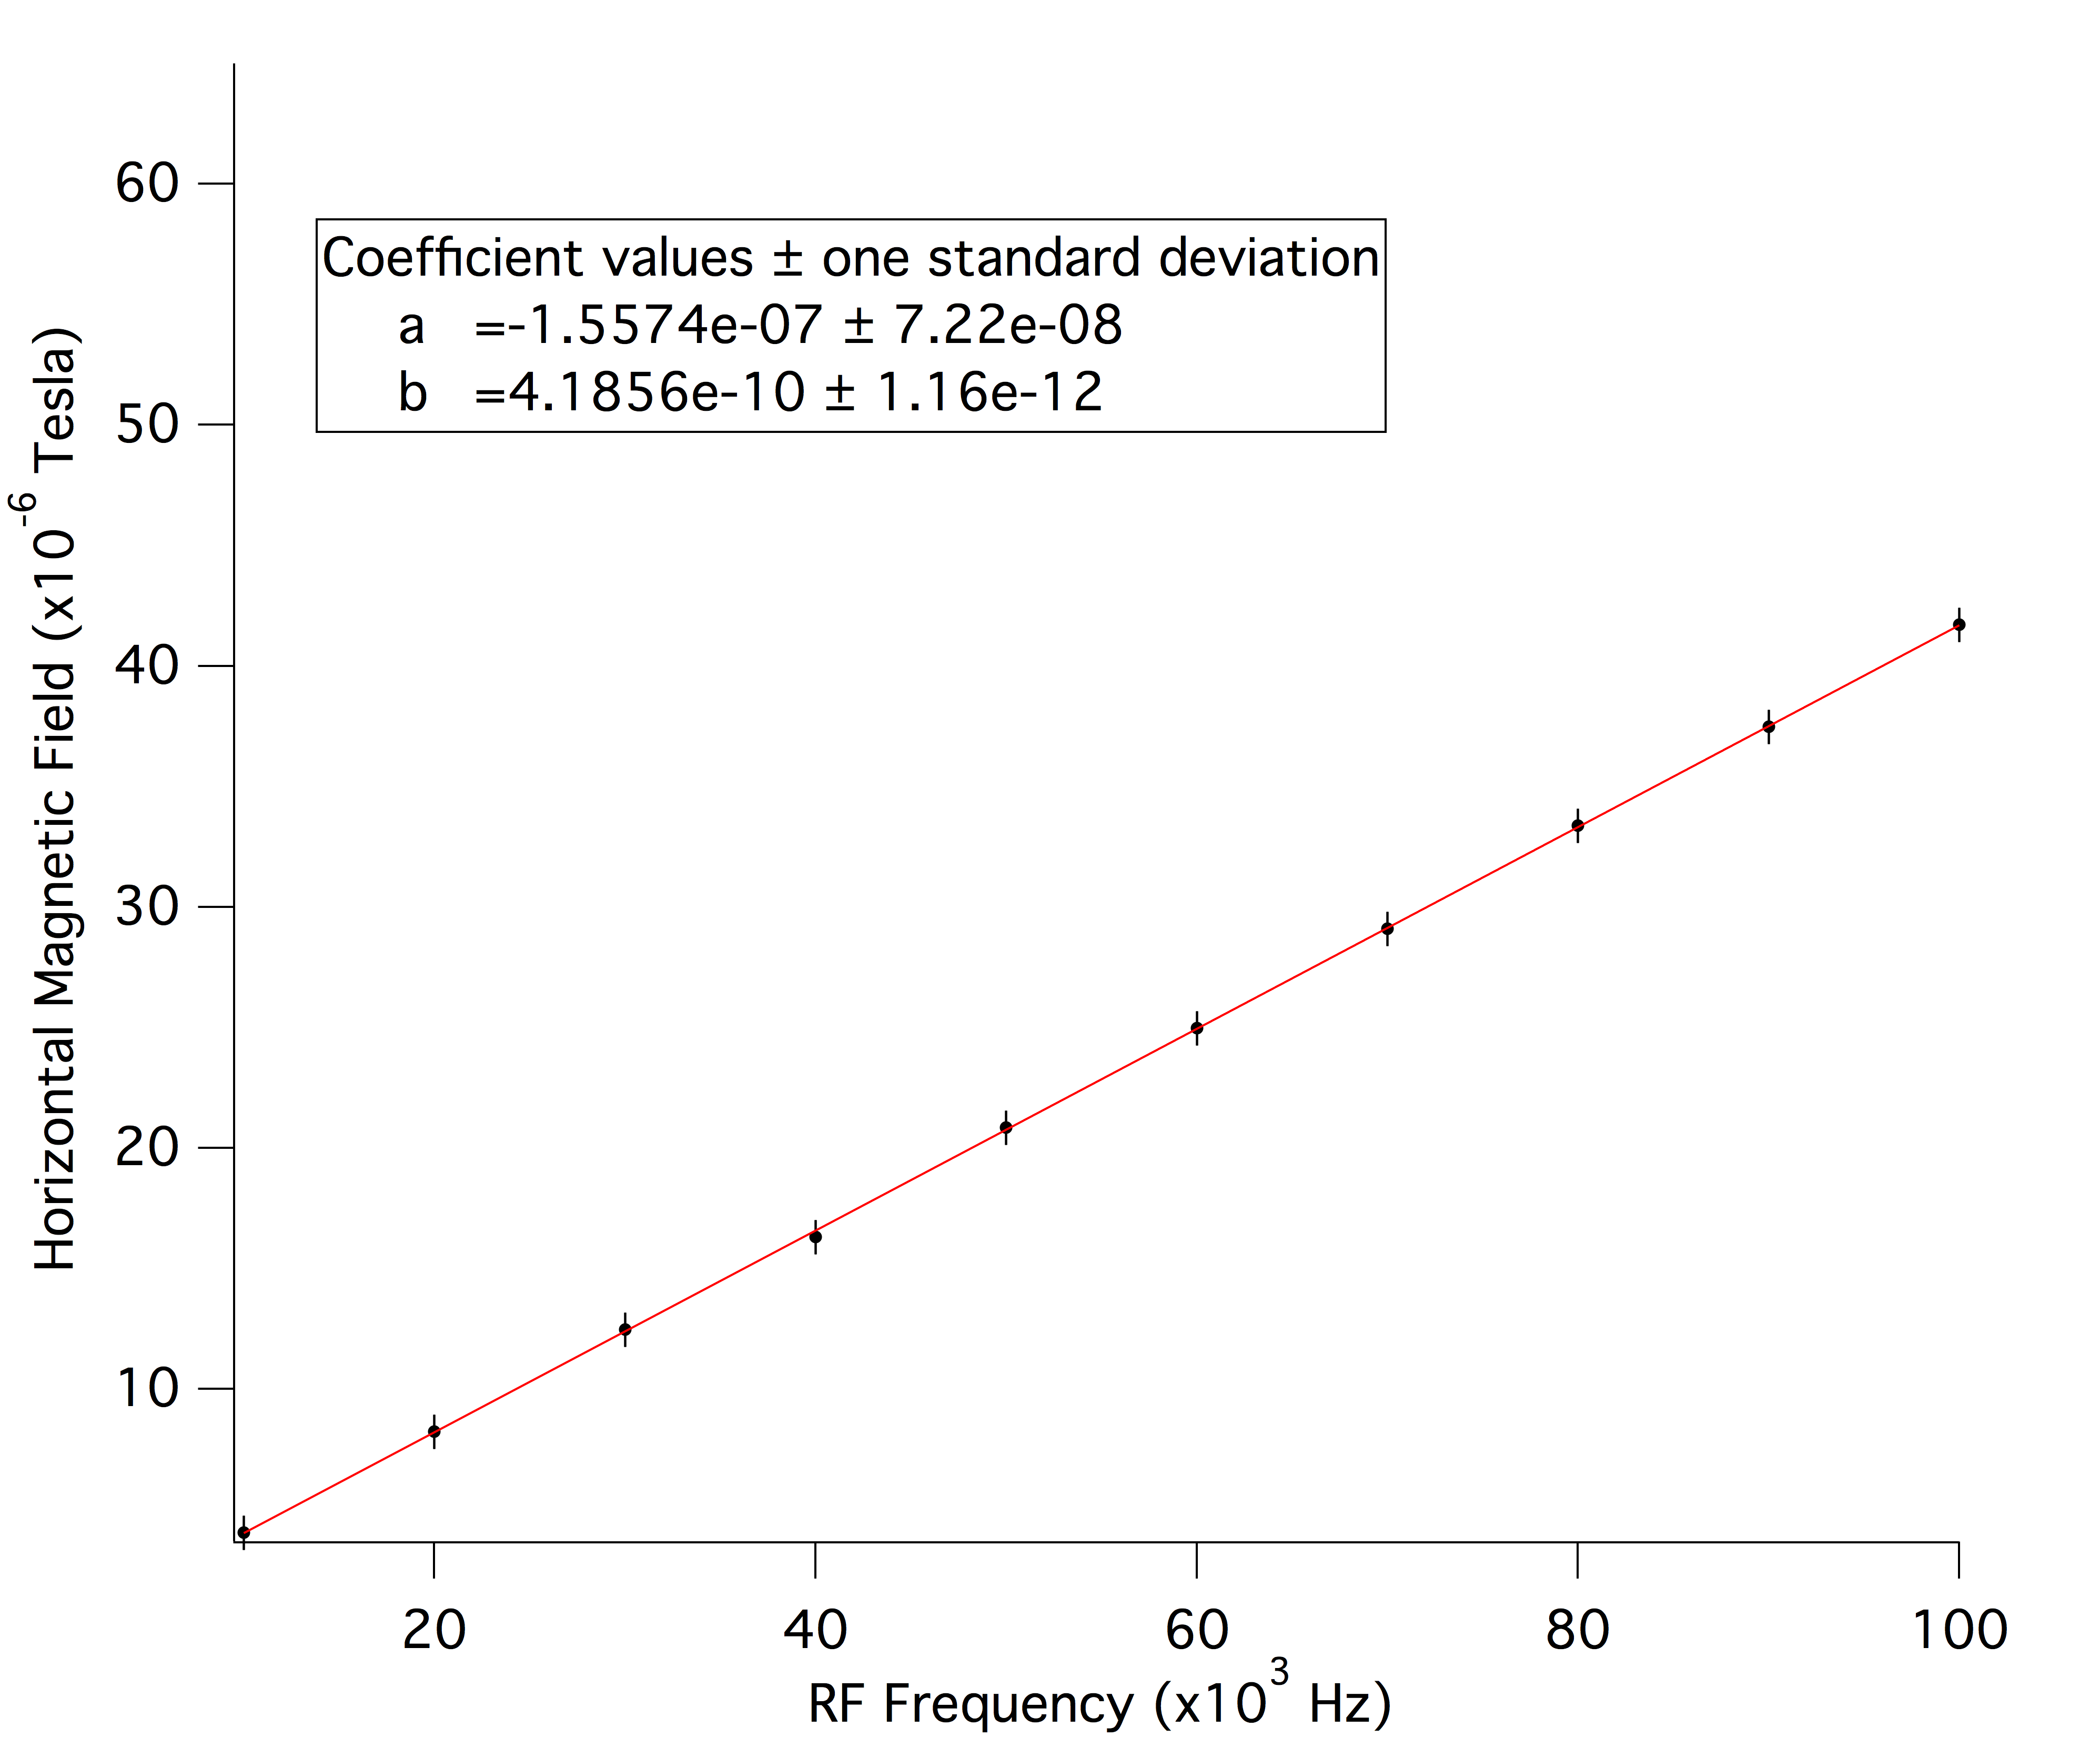
\includegraphics[width=8cm]{87vsFreq.png}
\caption{Horizontal magnetic field strength at 100 kHz. The left trough is the zero field resonance, the middle trough is RF absorption for $^87$Rb and the right trough is for Rb.}
\label{exp}
\end{figure}

%\begin{table}[h]
%\centering
%\caption{Single-slit data}
%\begin{ruledtabular}
%\begin{tabular}{ l c c c}
%Name & Symbol & Value & Uncertainties($\pm$)\\
%\hline
%Slit width & a & 93.9 $\mu m$ & 0.2 $\mu m$\\
%Wavelength & $\lambda$ & 0.67 nm & N/A \\
%Max voltage & $V_0$ & 1.350 V & 0.002 V\\
%Voltage offset & $V_{offset}$ &  0.004 V & 0.001 V\\
%Theta offset &$ \theta_{offset}$ & 1E-05 rad & 7E-06 rad \\
%\hline
%Chi Squared & $\chi^2$ & 1.56815 &
%\end{tabular}
%\end{ruledtabular}
%\label{data}
%\end{table}

%____________Discussion____________________________________________
\section{Discussion}

%____________Conclusion____________________________________________
\section{Conclusion}


\begin{acknowledgments}

We gratefully acknowledge Nathanael Fortune and Dana Parsons, who helped with the experimentation and editing of this experiment.  This work was supported by the Smith College Physics Department.

\end{acknowledgments}


\begin{thebibliography}{99}

%\bibitem{wik} Double Slit Experiment, \url{<http://upload.wikimedia.org/wikipedia/commons/c/c2/Single_slit_and_double_slit2.jpg/>}.
\bibitem{teach} TeachSpin Instructions Manual,\textit{Optical Pumping of Rubidium OP1-A}, 6/2002.

\end{thebibliography}

%\newpage   % Start a new page for tables

\end{document}
